\section{Introduction}
It is proposed to build a detector in order to verify the GEANT4 simulations while providing a framework to test light transport collection, spacing, and material properties in order to build a scaled modeled of a layered RPM8 detector.

There are serveral design parameters which must be determined ~\ref{fig:DetectorParameterSchematic}
\begin{itemize}
    \item detector material,
    \item detector thickness,
    \item detector encapsulating material,
    \item detector encapsulating material thickness,
    \item and spacing between layers.
\end{itemize}
\begin{figure}
    \centering
    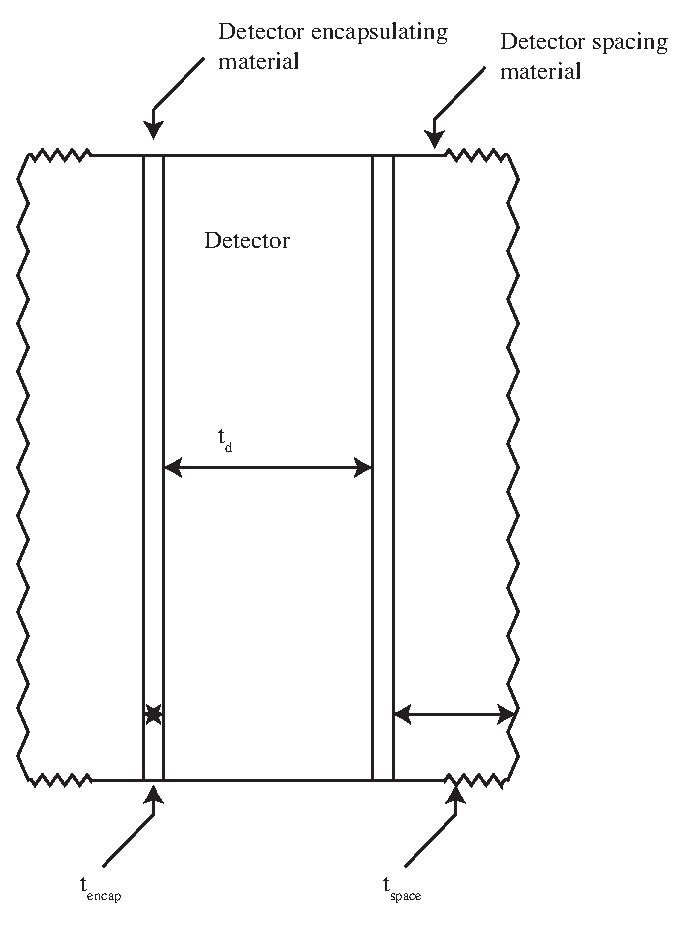
\includegraphics[]{ThinFilmDetectorDesign}
    \caption{Detector Design Parameters}
    \label{fig:DetectorParameterSchematic}
\end{figure}

\subsection{Detector Material}
${}^6$LiF was chosen as the material of choice because of it's high light output ($16x10^4$ photons per neutron) and large ${}^{6}$LiF content \cite{carel_w.e_inorganic-scintillators_2001}. 
Innovative American Technologies (IAT) have perusued ${}^6$LiF:ZnS based detectors with mixed results.
The IAT detector is a LiF:ZnS coated paddle with two PMT's at either end of an assemply that is 12" x 5" x 85" (size of RPM8)~\ref{fig:IATPaddle}.
The neutron efficiency was reported by the manufacture to be 3.7 cps per ng ${}^{252}$Cf, with a gamma sensitivity of less than $10^{-7}$ in a > 20mR per hr gamma field.  The GARRn was within the criteria.
Previous models tested at PNNL in 2010 were scaled models which did not have an adquate neutron count rate but passed the other criteria \cite{kouzes_lithium_2010}.
\begin{figure}
    \centering
    \includegraphics[width=\textwidth]{IAT_NDM_4-0}
    \caption{IAT NDM 4.0 ${}^6$LiF:ZnS neutron detector (12" x 5" x 85")}
    \label{fig:IATPaddle}
\end{figure}

Eljen Technology (Sweetwater, TX) provides two ${}^6$LiF:ZnS screens, the EJ-426-0 and EJ-426-HD2 with backing materials constining of 50 $\mu$m of aluminum foil, 0.12 mm of aluminzied mylar, a 0.5 mm aluminum sheet, a 0.4 mm sheet of highly relrective alumin, and 0.25 mm of clear polyester with the option of a 1 mm acrylic plate \cite{_ej-426_2012}.
It was decided to use EJ-426-HD2 because it contains 1.6 times the ${}^{6}$Li content as EJ-426-0. EJ-426 has a ${}^{6}$Li atomic density of $1.39\times10^{22}$ atoms of ${}^6$Li per cm${}^3$ \cite{_ej-426_2012}. EJ-426 is opaque, however, due to the ZnS.  In addition previous experianced with EJ-426 a slight brittleness was observed.
